\section{Component View on Architecture}

Lustre is a GNU General Public licensed, open-source distributed parallel
filesystem developed and maintained by Sun Microsystems Inc. Due to the
extremly scalable architecture of the Lustre filesystem, Lustre deployments
are popular in scientific supercomputing, as well as in the oil and gas,
manufacturing, rich media, and finance sectors. Lustre presents a POSIX
interface to its clients with parallel access capabilities to the shared file
objects. As of this writing, 15 of the top 30 fastest supercomputers in
the world use Lustre filesystem for high-performance scratch space.

Lustre is an object-based filesystem. It is composed
of three components: Metadata servers (MDSs), object storage servers (OSSs),
and clients.  Figure~\ref{fig:lustre-arch} illustrates the Lustre
architecture.  Lustre uses block devices for file data and metadata storages
and each block device can be managed by only one Lustre service. The total
data capacity of the Lustre filesystem is the sum of all individual OST
capacities.  Lustre clients access and concurrently use data through the
standard POSIX I/O system calls. 

\begin{figure}[hhhh]
     \begin{center}
             \resizebox{0.8\linewidth}{!}{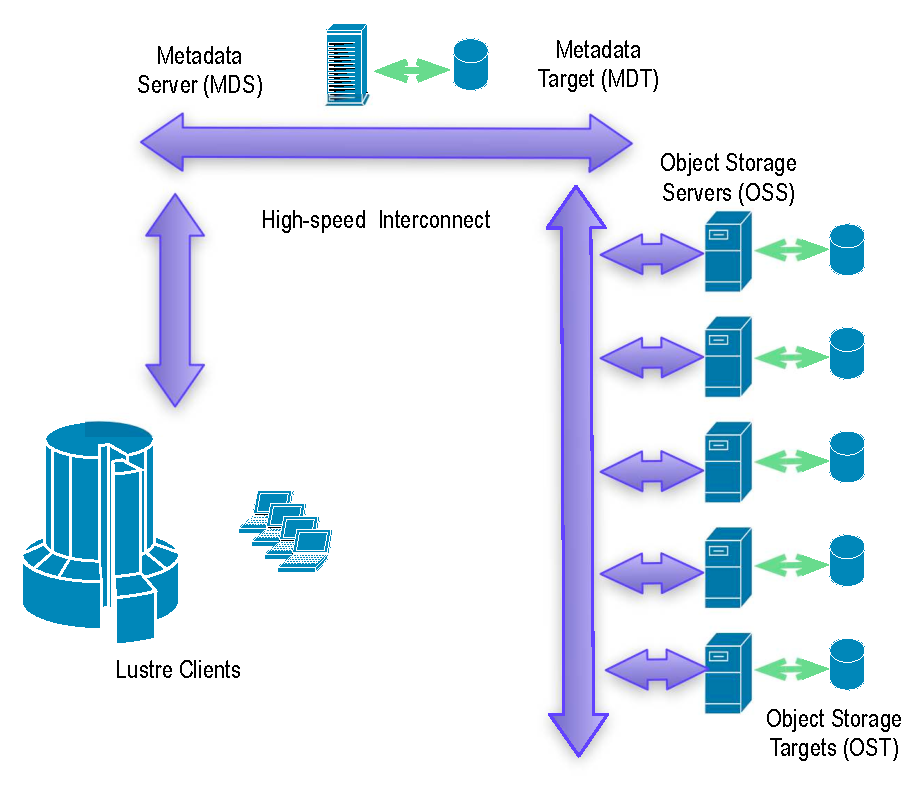
\includegraphics[scale=0.7]{img/lustre-arch}}
             \caption{Lustre components.}
             \label{fig:lustre-arch}
     \end{center}
\end{figure}

%
%At component level, Lustre system can be organized into three major pieces:
%Lustre client, Lustre server fronts (MDS/MGS, and OSS/OST) and Luster server
%backend (fsfilt and ldiskfs). In a nutshell:
%

\begin{itemize}

\item MDS (metadata servers) provides metadata services. Correspondingly, an
MDC (metadata client) is a client of those services. One MDS per filesystem
manages one metadata target (MDT). Each MDT stores file metadata, such as file
names, directory structures, and access permissions.

\item MGS (management server) serves configuration information of the Lustre
filesystem.

\item OSS (object storage server) exposes block devices and serves data.
Correspondingly, OSC (object storage client) is client of the services. Each
OSS manages one or more object storage targets (OSTs), and OSTs store file
data objects. 

\end{itemize}

The collection of MDS/MGS and OSS/OST are sometimes referred to as
\textit{Lustre server fronts}, fsfilt and ldiskfs as \textit{Luster server
backends}. In the following discussion, we start from the Lustre client side,
and follow the general data and control thread all the way to the OST and MDS.
The discussion touches on many components while skipping details to make the
structural relationship more obvious. 

\subsection*{Lustre Client}

Lustre, being a POSIX-compliant filesystem, presents a unified filesystem
interface such as open(), read(), write(), etc. to the user. In Linux, this
unified interface is achieved through Virtual File System (VFS) layer (in
BSD/Solaris, this would be known as~\url{vnode} layer). There is a shim layer
in Lustre called \textbf{llite} that is hooked with VFS to present that
interface. The file operation requests that reach llite will then go through
the whole Lustre software stack to access the Lustre filesystem, as shown in
Figure~\ref{fig:lustre_components}.

\begin{figure}[htb]
\centering
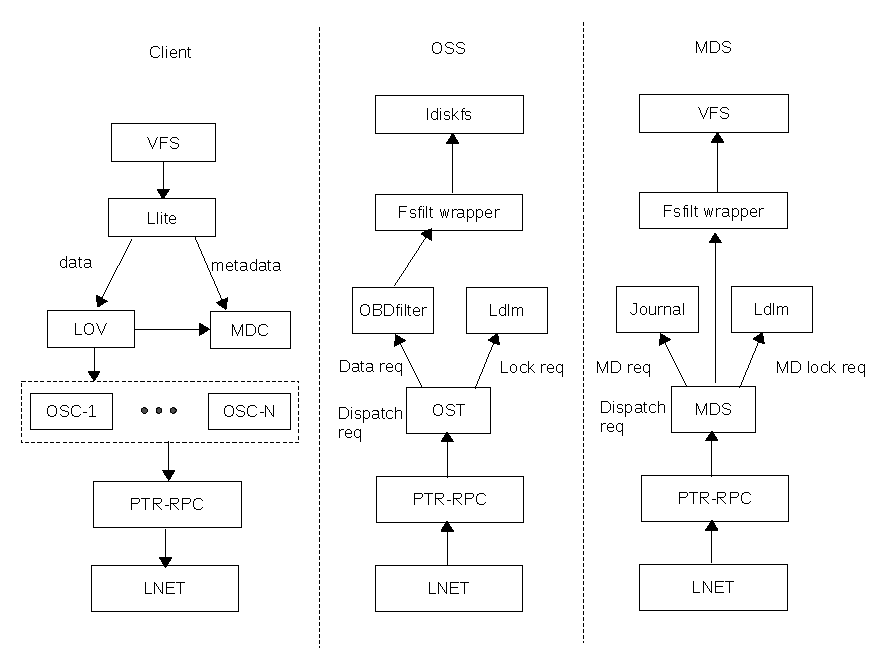
\includegraphics[width=4.5in]{img/lustre_components}
\caption{A component view of Lustre architecture.}
\label{fig:lustre_components}     
\end{figure}
 
In Lustre, general file operations such as create, open, read, etc. require
metadata information stored on \textbf{MDS}. This service is accessed through
a client interface module, known as \textbf{MDC}.

From the MDS point of view, each file is composed of multiple data objects striped
on one or more OSTs. A file object's layout information is defined in the
extended attribute (EA) of the inode. Essentially, EA describes the mapping
between file object id and its corresponding OSTs. This information is also
known as \textit{striping EA}.

For example, if file A has a stripe count of three , then its EA might look like:

\begin{Verbatim}
    EA ---> <obj id x, ost p>
            <obj id y, ost q>
            <obj id z, ost r>
            stripe size and stripe width
\end{Verbatim}

So if the stripe size is 1MB, then this would means that [0,1M), [4M,5M) ... are
stored as object $x$, which is on OST $p$; [1M, 2M), [5M, 6M) ... are stored as
object y, which is on OST $q$; [2M,3M), [6M, 7M) ... are stored as object $z$,
which is on OST $r$.

Before reading the file, client will query the \textbf{MDS} via MDC and be
informed that it should talk to \url{<ost p, ost q, ost r>} for this
operation.  This information is structured in so-called LSM, and client side
\textbf{LOV} (logical object volume) is to interpret this information so
client can send requests to OSTs.  Here again, the client communicates with OST
through a client module interface known as OSC. Depending on the context, OSC
can also be used to refer to an OSS client by itself.

All client/server communications in Lustre are coded as an RPC request and
response.  Within the Lustre source, this middle layer is known as Portal RPC, or
\textbf{ptl-rpc}: It translates and interprets filesystem requests to and
from the equivalent form of RPC request and response, and the \textbf{LNET} module to
finally put that down onto the wire.

\subsection*{OSS}

At the bottom of the OSS stack, are the familiar LNET and Portal-RPC
layers. As with the client side stack, Portal RPC will interpret the request.  The
important thing to bear in mind is that the requests handled by OSS are data
requests \footnote{As well as some size requests, such as glimpse requests from a
client}, not metadata requests. Metadata requests should be passed on and
handled by MDS stack, as shown at the rightmost column in
Figure~\ref{fig:lustre_components}.

Going up on the stack, \textbf{OST} acts like a dispatcher: it invokes
different functions based on the type of request. Broadly speaking, there are
two types of request: \textit{lock} related and \textit{data} related. The
former will be passed onto \textbf{ldlm} (Lustre distributed lock manager) to
handle and the latter will go to \textbf{obdfilter}.  The obdfilter is a module
that interconnects the Lustre stack and the regular OS stack, so to speak. It
defines a generic API that translates a Lustre-specific request to the
backend filesystem-specific request, with the help another wrapper API
component called \textbf{fsfilt}. Conceptually, fsfilt is like a VFS layer, if
you register proper file operations with it, it will use the particular
filesystem as the backend; in the case of Lustre, this backend filesystem
is currently \textbf{ldiskfs}. In the future, ZFS will be supported as backend
filesystem as well, and fsfilt could probably be redesigned or replaced by a
better filesystem-agnostic middle layer.

\subsection*{MDS}

The MDS software stack is similar to the OSS stack but, there are some
differences between them. The main difference is that the MDS software stack
does not have an obdfilter as can be seen in Figure
\ref{fig:lustre_components}. The dispatcher is called~\textbf{MDS}. Of course,
it does more than just dispatch, and it will be explained in detail in Section
\ref{sec:lustre-mdc}. For a metadata change request, MDS will do journaling a
bit differently: it will start a transaction before directly invoking the VFS
API. The particular component block may be called \textbf{dcache} as it mostly
concerns operating on a \textbf{dentry} cache, but in a larger framework, it is
really part of the VFS.

